\chapter{Testování}

\subsection{Naměřená data pro řízení podle teplotních plánů}

Bylo provedeno měření teplotních plánů. Cílem bylo zjistit, jak dochází ke zpoždění vytápění na požadovanou teplotu vůči nastavenému časovému plánu. Měření bylo provedeno pro období 19.~11.~2021 od 00:00 do 21 . 11. 2021 do 20:00 pro teplotní plán místnosti „Ložnice rodičů“ (obrázek~\ref{fig:teplotni-plan-loznice-rodicu}). Teplotní úseky pro tento teplotní plán jsou od 00:00–06:30, 06:30–17:00 a 17:00–00:00.

\begin{figure}[H]
    \centering
    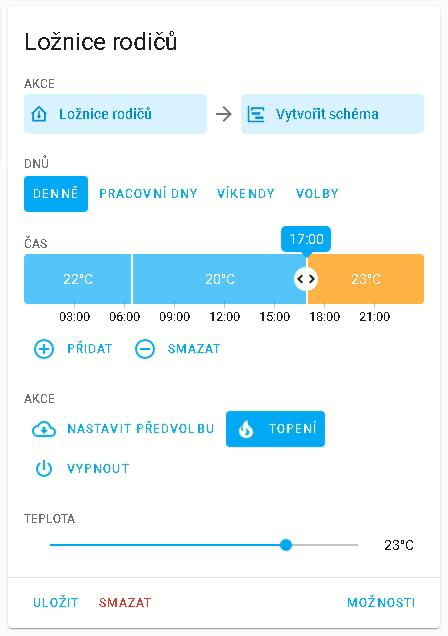
\includegraphics[width=0.5\textwidth]{images/testovani/teplotni-plany/teplotni-plan-loznice-rodicu.png}
    \caption{Teplotní plán pro místnost „Ložnice rodičů“}
    \label{fig:teplotni-plan-loznice-rodicu}
\end{figure}

Na následujících grafech je průběh pro aktuální teplotu (modrá křivka), požadovanou teplotu (fialová křivka) a stav topení (oranžová křivka). Na obrázku \ref{fig:loznice-rodicu-termostat-zacatek-vytapeni} je začátek vytápění podle teplotního plánu v intervalu od 17:00–00:00. Podle grafu je aktuální teplot 22 °C, cílová je 23 °C. Této požadované teploty se dosáhne přibližně v čase 19:00 (obrázek \ref{fig:loznice-rodicu-termostat-konec-vytepeni}), zpoždění 2 hodiny vůči začátku časového úseku. Dále podle obrázku \ref{fig:loznice-rodicu-termostat-presazeni-teploty} je vidět setrvačnost podlahového vytápění, která způsobí zvýšení teploty až na 23,5 °C.



\begin{figure}[H]
    \centering
    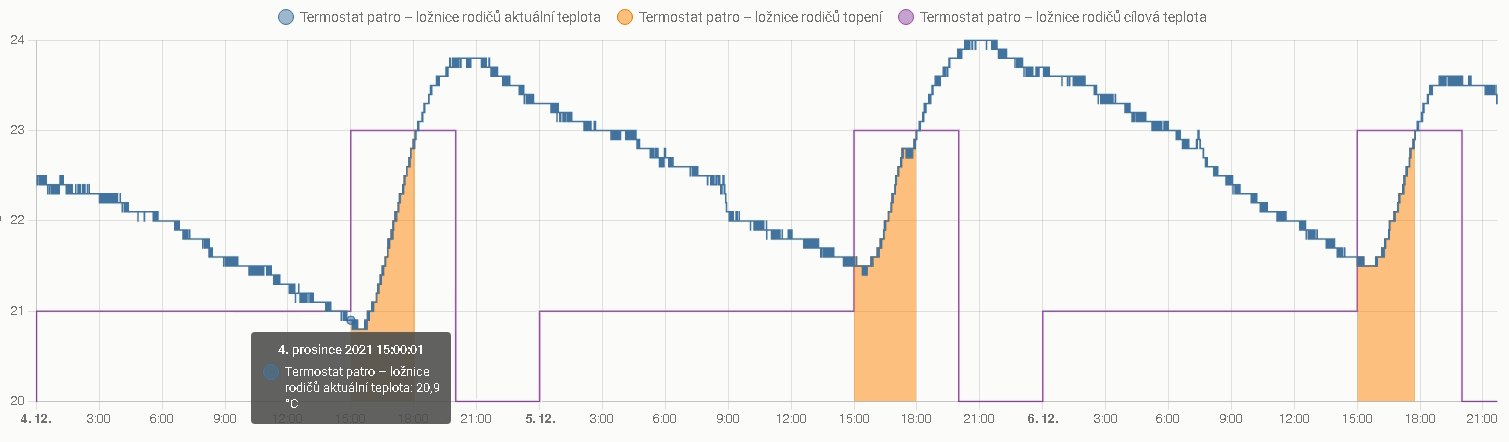
\includegraphics[width=\textwidth]{images/testovani/teplotni-plany/loznice-rodicu-termostat-zacatek-vytapeni.png}
    \caption{Začátek vytápění v 17:00 pro teplotní úsek 17:00–00:00.}
    \label{fig:loznice-rodicu-termostat-zacatek-vytapeni}
\end{figure}

\begin{figure}[H]
    \centering
    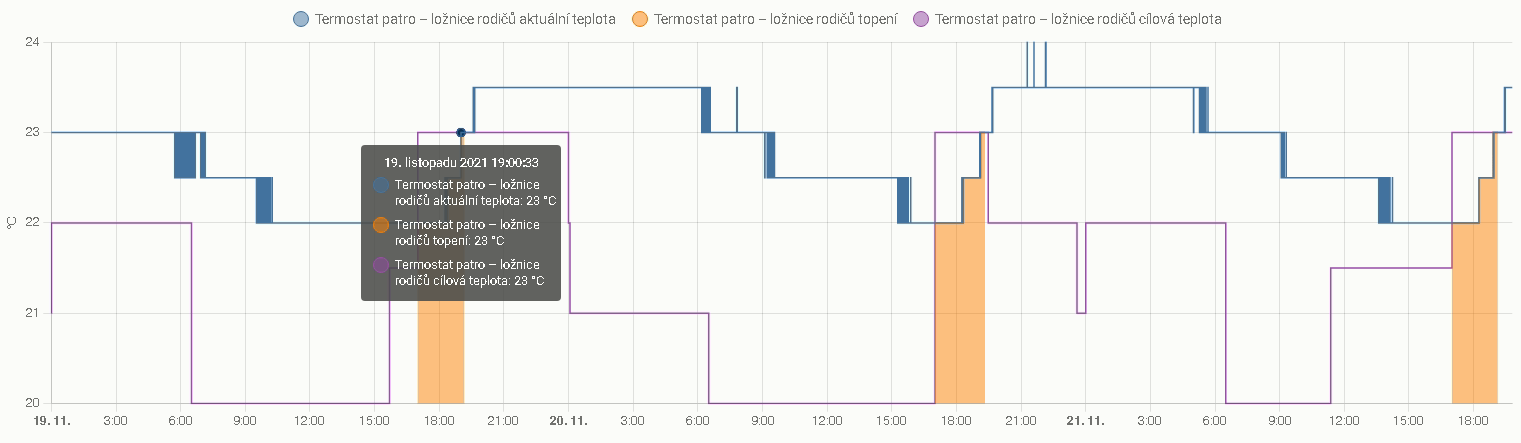
\includegraphics[width=\textwidth]{images/testovani/teplotni-plany/loznice-rodicu-termostat-konec-vytepeni.png}
    \caption{Dosažení požadované teploty přibližně v 19:00.}
    \label{fig:loznice-rodicu-termostat-konec-vytepeni}
\end{figure}

\begin{figure}[H]
    \centering
    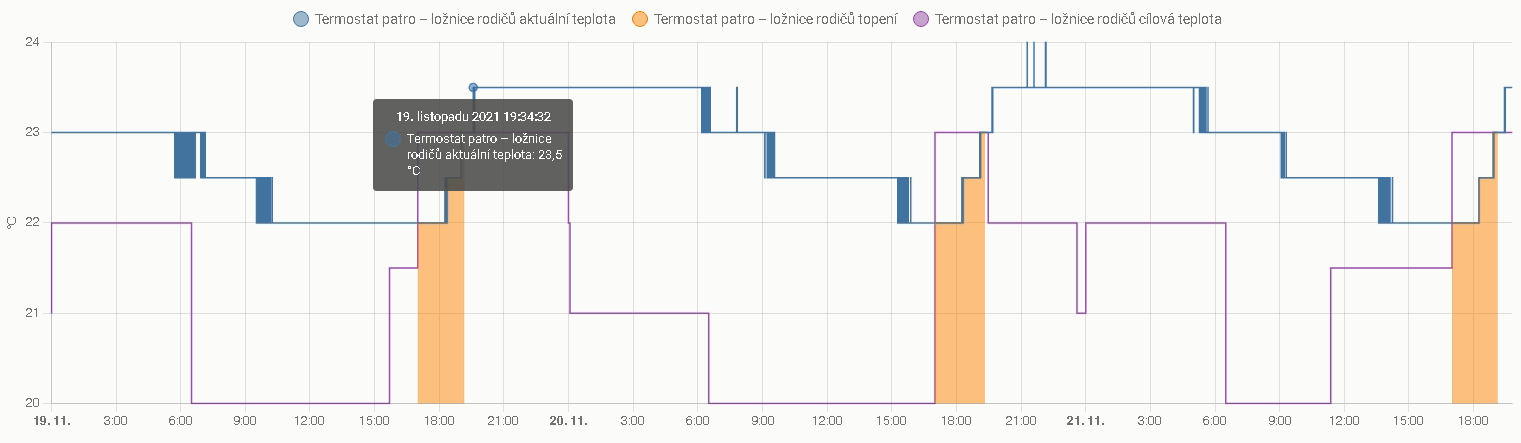
\includegraphics[width=\textwidth]{images/testovani/teplotni-plany/loznice-rodicu-termostat-presazeni-teploty.png}
    \caption{Přetopení místnost způsobené setrvačností podlahového vytápění.}
    \label{fig:loznice-rodicu-termostat-presazeni-teploty}
\end{figure}

\subsection{Naměřená data pro řízení podle teplotních plánů s úpravou předpovědi počasí}